%
%	Begrifflichkeiten
%

\pagebreak
\section{The need for Governance and Security in container run-time environments}

\onehalfspacing

\subsection{Container run-time environments}

Let's start with the basics. In most of IT, Kubernetes\footnote{See \textit{The Linux Foundation (2020)}: Production-Grade Container Orchestration. \cite{kubernetes}} has emerged as the container run-time environment of choice.

Earlier competitors, such as Docker Swarm or Mesos DC/OS, have all but vanished.

The original platforms that spawned cloud-native computing and application design and gave us the concept of micro-services, Heroku and Cloud Foundry, have also slightly gone out of favor, or, in the case of Cloud Foundry, moved to a Kubernetes-based run-time.

\subsection{Kubernetes Architecture}

A Kubernetes container run-time environment, or cluster, in general will consist of one or more logically grouped systems. These systems can be either physical nodes or better, be virtualized, and all of them run a supported container run-time, such as Docker or Podman.

A Kubernetes cluster consists of one or more Master nodes, the so-called Control Plane, and one or more worker nodes, the Execution Plane. Most commonly, there are three nodes in the control plane, and three or more nodes in the execution plane, sometimes with different sizing or capabilities. An odd number of nodes should be chosen for the control plane, because the underlying etcd database is a distributed system and needs to reach quorum on startup.

The Kubernetes control plane takes care of orchestrating the application deployments and maintains their state; the worker nodes on the other execute the actual application containers as defined and scheduled by the control plane.

Kubernetes, in itself, is also a containerized application.

In addition to providing compute nodes, Kubernetes also provides an overlay network that allows communication between the cluster nodes, invisible to the outside world, and ingress controllers for inbound network access to the running applications. Persistent storage, even though it's an anathema to stateless, cloud-native computing, is provided through persistent volumes and storage classes.

All administrative access to a given Kubernetes cluster is via the master nodes and its Kubernetes API endpoint.

\subsection{Kubernetes Security}

Installing the first Kubernetes cluster is not a big task anymore, especially on the three big public cloud providers, which all offer managed Kubernetes clusters with easy, one-click installations.

Designing the platform landscape, however, does need some architectural knowledge and should be planned well in advance.

One of the crucial components of security when running containers in production, according to NIST, is the separation in between applications and systems. Careful consideration should be put on the number and type of Kubernetes clusters deployed.\footnote{See \textit{Weibel, D. (2020)}: Architecting Kubernetes clusters. \cite{howMany}}

Kubernetes itself, at the time of writing, does not provide for hard tenancy. To entirely separate applications on all layers (compute, network, and storage), the use of multiple clusters is a good option. Many enterprises might thus end up with more than one Kubernetes cluster, sometimes with many more, which will, in turn, have a significant effect on operations.

With the increase in popularity, Kubernetes also brings new security challenges that should be considered when designing the IT environment.\footnote{See \textit{Weizmann, Y. (2020)}: Threat matrix for Kubernetes . \cite{threatMatrix}}

We're observing a trend in Enterprise IT to move from traditional perimeter-based network security to more modern zero- or low-trust networks with identity-based security and temporary infrastructure. Having multiple, short-lived Kubernetes cluster is a likely scenario going forward.

\subsection{Rancher overview}

What is Rancher? According to the Rancher Labs website, it is "[...] a complete software stack for teams adopting containers. It addresses the operational and security challenges of managing multiple Kubernetes clusters, while providing DevOps teams with integrated tools for running containerized workloads"\footnote{\textit{Rancher Labs (2019)}: Run Kubernetes Everywhere. \cite{rancher}}

Rancher provides a management platform to centrally manage multiple Kubernetes clusters in Enterprise IT, all from a choice of two user-friendly GUIs. Rancher also offers integration tools for application development and robust enterprise-grade features for security and governance. For operations, Rancher provides integrated solutions for logging, monitoring, and auditing, together with many other features.

The classic Rancher GUI looks like this:

\begin{figure}[H]
\centering
\caption {Rancher Overview}
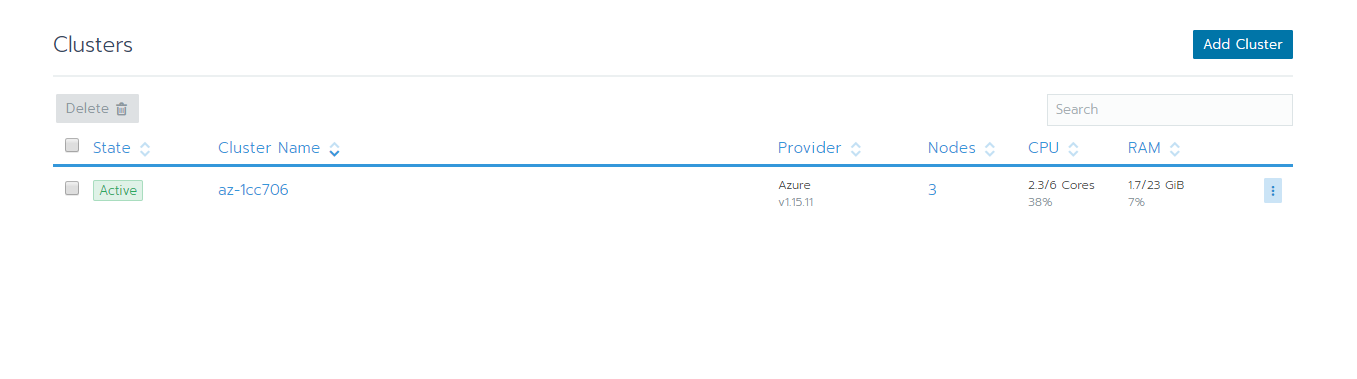
\includegraphics[width=\linewidth]{images/cluster-overview.png}
\label{fig:rancherOverview}
\end{figure}

\subsection{Rancher Architecture}

Rancher is, similar to Kubernetes, itself a containerized application and can be installed from a single image to a single Docker host. Such a single-node installation is ideal for testbeds or local Rancher installations on a laptop, for example. A single node installation does not provide any redundancy in case of failure.

For production installations, Rancher can be installed on a Kubernetes cluster, using Kubernetes' redundancy mechanisms for high-availability and resiliency. It could either be co-hosted on an existing cluster or better, on a small, separate infrastructure cluster. It is good practice in IT to keep administrative tools on separate infrastructure from the administered infrastructure, and thus the installation on a different cluster is the most widespread.

In addition to the GUI, the Rancher server also provides a central Kubernetes API endpoint, which acts as an intermediary between the users and the actual Kubernetes clusters.

More details on the Rancher architecture can be found the technical architcure document.\footnote{See \textit{Rancher Labs (2020)}: Rancher Technical Architecture. \cite{technicalArchitecture}}
